%% V1.0
%% by Gabriel Garcia, gabrcg@gmail.com
%% This is a template for Udacity projects using IEEEtran.cls

%% Be Udacious!

\documentclass[10pt,journal,compsoc]{IEEEtran}

\usepackage[pdftex]{graphicx}    
\usepackage{cite}
\hyphenation{op-tical net-works semi-conduc-tor}


\begin{document}

\title{Map My World}

\author{Jeremy Hale}

\markboth{SLAM, Robotics Nanodegree Program, Udacity}%
{}
\IEEEtitleabstractindextext{%

\begin{abstract}
The Udacity Robotics Nanodegree project Map My World is a simluation of a small robot mapping two different environments. The robot uses a RGBD camera and a laser scanner with the RTAB-Map method of SLAM (simultaenous localization and mapping) to create a map of the environments. ROS and Gazebo/RViz are the main tools employed.
\end{abstract}

% Note that keywords are not normally used for peerreview papers.
\begin{IEEEkeywords}
Robot, IEEEtran, Udacity, \LaTeX, Localization.
\end{IEEEkeywords}}


\maketitle
\IEEEdisplaynontitleabstractindextext
\IEEEpeerreviewmaketitle
\section{Introduction}
\label{sec:introduction}

\IEEEPARstart{T}{his} project demonstrates the use of SLAM in simulation using ROS and specifically the RTAB-Map implementation of SLAM. SLAM is a technique to solve the problem of localization while building a map from sensor inputs. In this simulation, a small two-wheel robot with RBGD camera and laser scanner is manually navigated around an environment. During navigation, the robot uses its sensor inputs to build a map of the environment.

The problem of mapping applies to many different situations as a robot may commonly find itself in an environment for which it does not have a map a priori. Even if a map were to exist, most environments in the world are not static. In homes and offices, for example, furniture or other significant objects or obstructions may be moved and would differ from prior maps.

\section{Background}
Explain the importance of both mapping two and three dimensional space.

Background - The student provides a sufficient background into the scope of the problem / technologically while also identifying some of the current challenges in robot mapping and why the problem domain is an important piece of robotics. They further discuss and compare mapping algorithms

\section{Model Configuration}
The robot was based on the Udacity robot from the "Where am I?" project. It was a small box-shaped chassis with 2 driven-wheels on the sides and 2 stabilizing wheels fore and aft. The robot has a Hokuyo laser scanner and a camera attached on the front. In the previous project, the camera was a simple RGB camera. This was changed to an RGBD camera to satisfy the project requirements.

\begin{figure}[thpb]
    \centering
    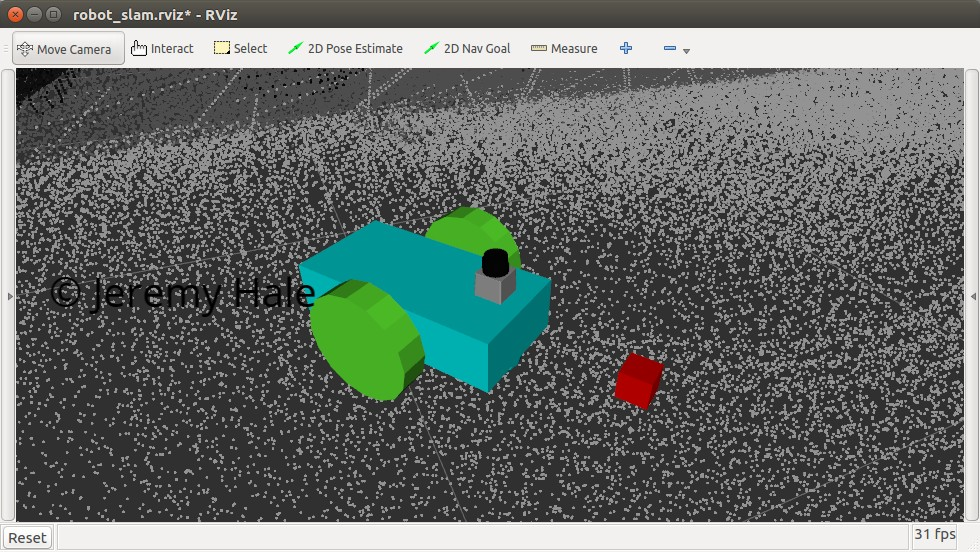
\includegraphics[width=\linewidth]{robot}
    \caption{Robot}
    \label{fig:robot}
\end{figure}

\begin{figure}[thpb]
    \centering
    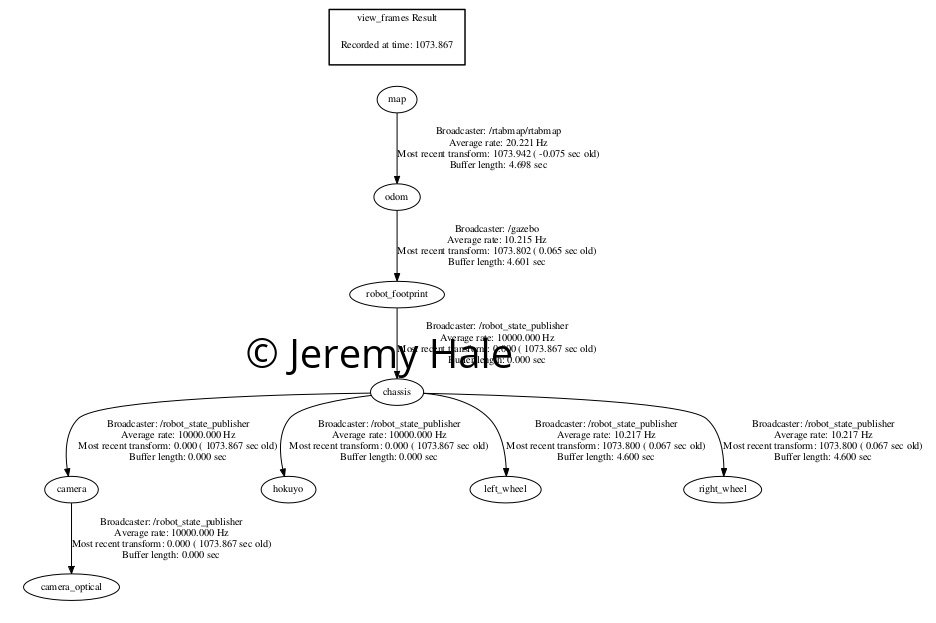
\includegraphics[width=\linewidth]{frames}
    \caption{TF Frames}
    \label{fig:frames}
\end{figure}


Scene and robot configuration - Student explains how the gazebo world was created by providing an overview of the layout of items in his/her customized Gazebo world. Student also describes the robot's parameters, sensor features, and reasoning on the package structure.

\section{World Creation}
The personal "world" is supposed to be a back alley. There is a large brick wall, a pickup truck, a dumpster and a fire hydrant.

\begin{figure}[thpb]
    \centering
    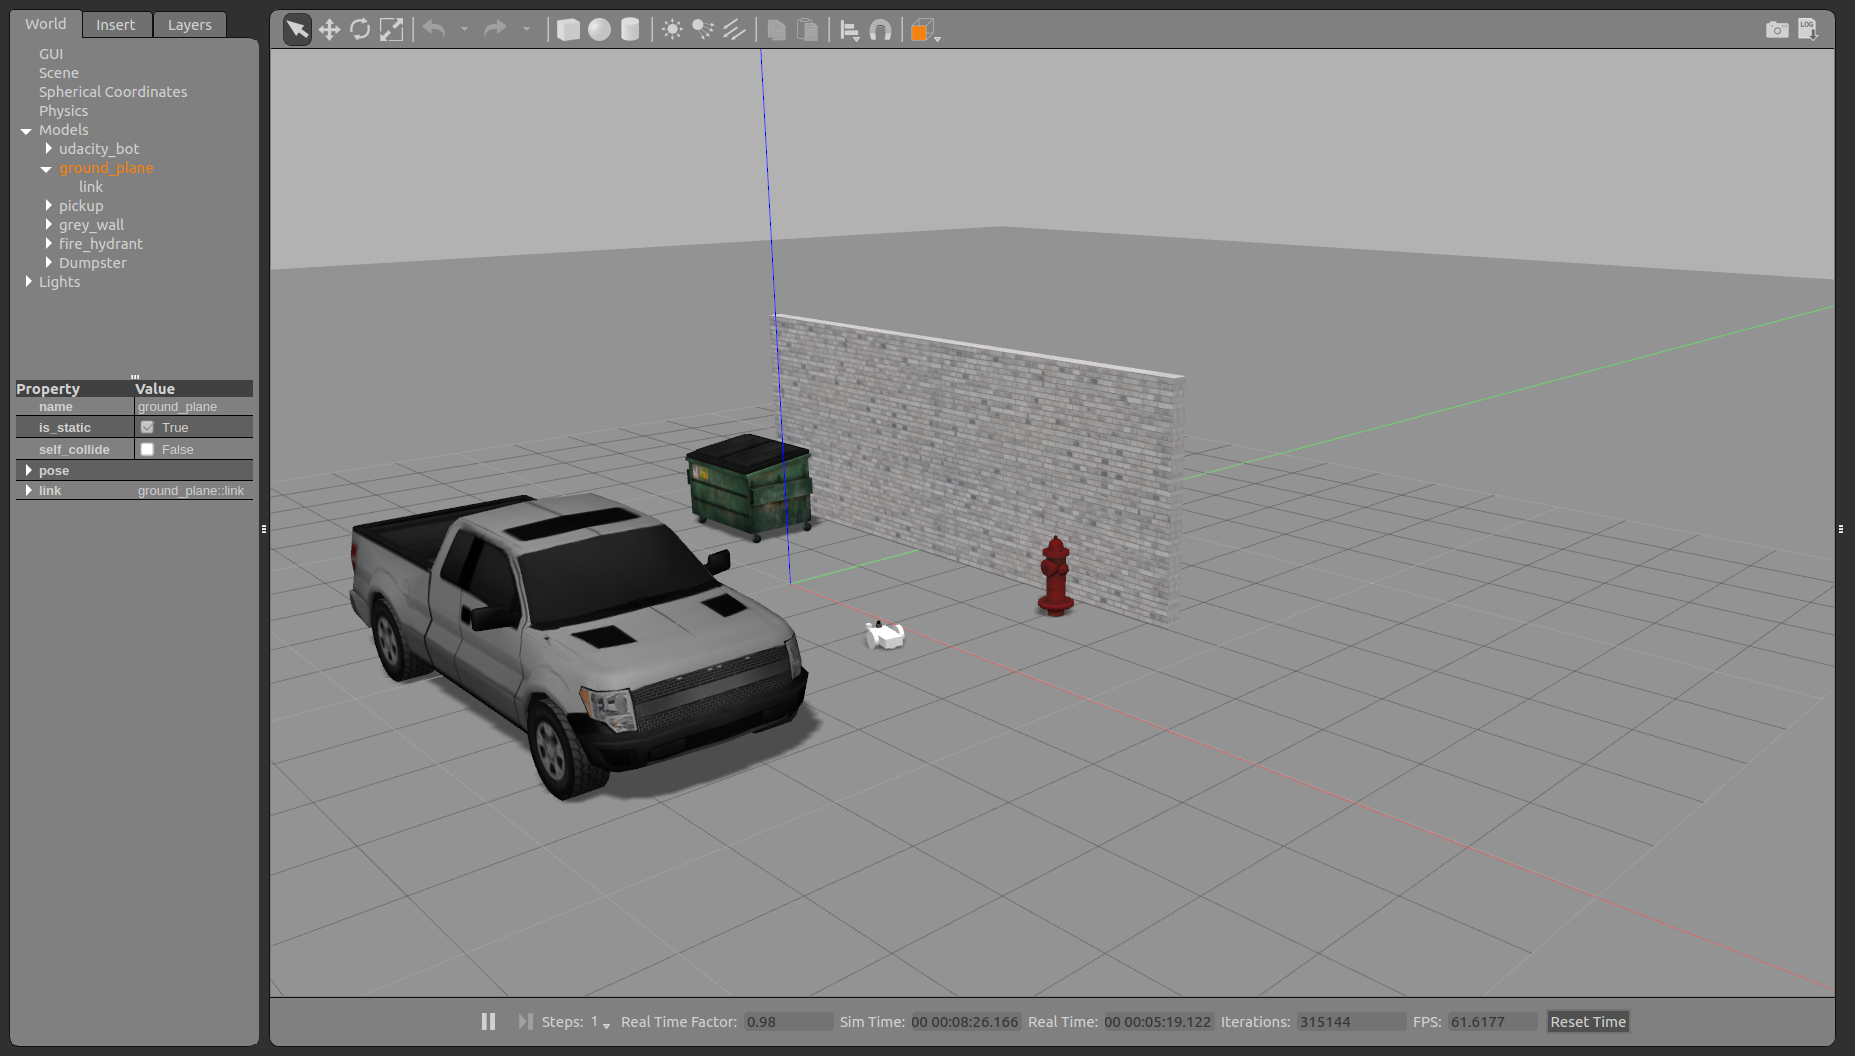
\includegraphics[width=\linewidth]{alley_gazebo}
    \caption{Alley}
    \label{fig:alley}
\end{figure}

\section{Results}

\subsection{Kitchen \& Dining}

The occupancy and 3D maps for the "Kitchen and Dining" world are shown below. There are also images showing the 3 closures.

\begin{figure}[thpb]
    \centering
    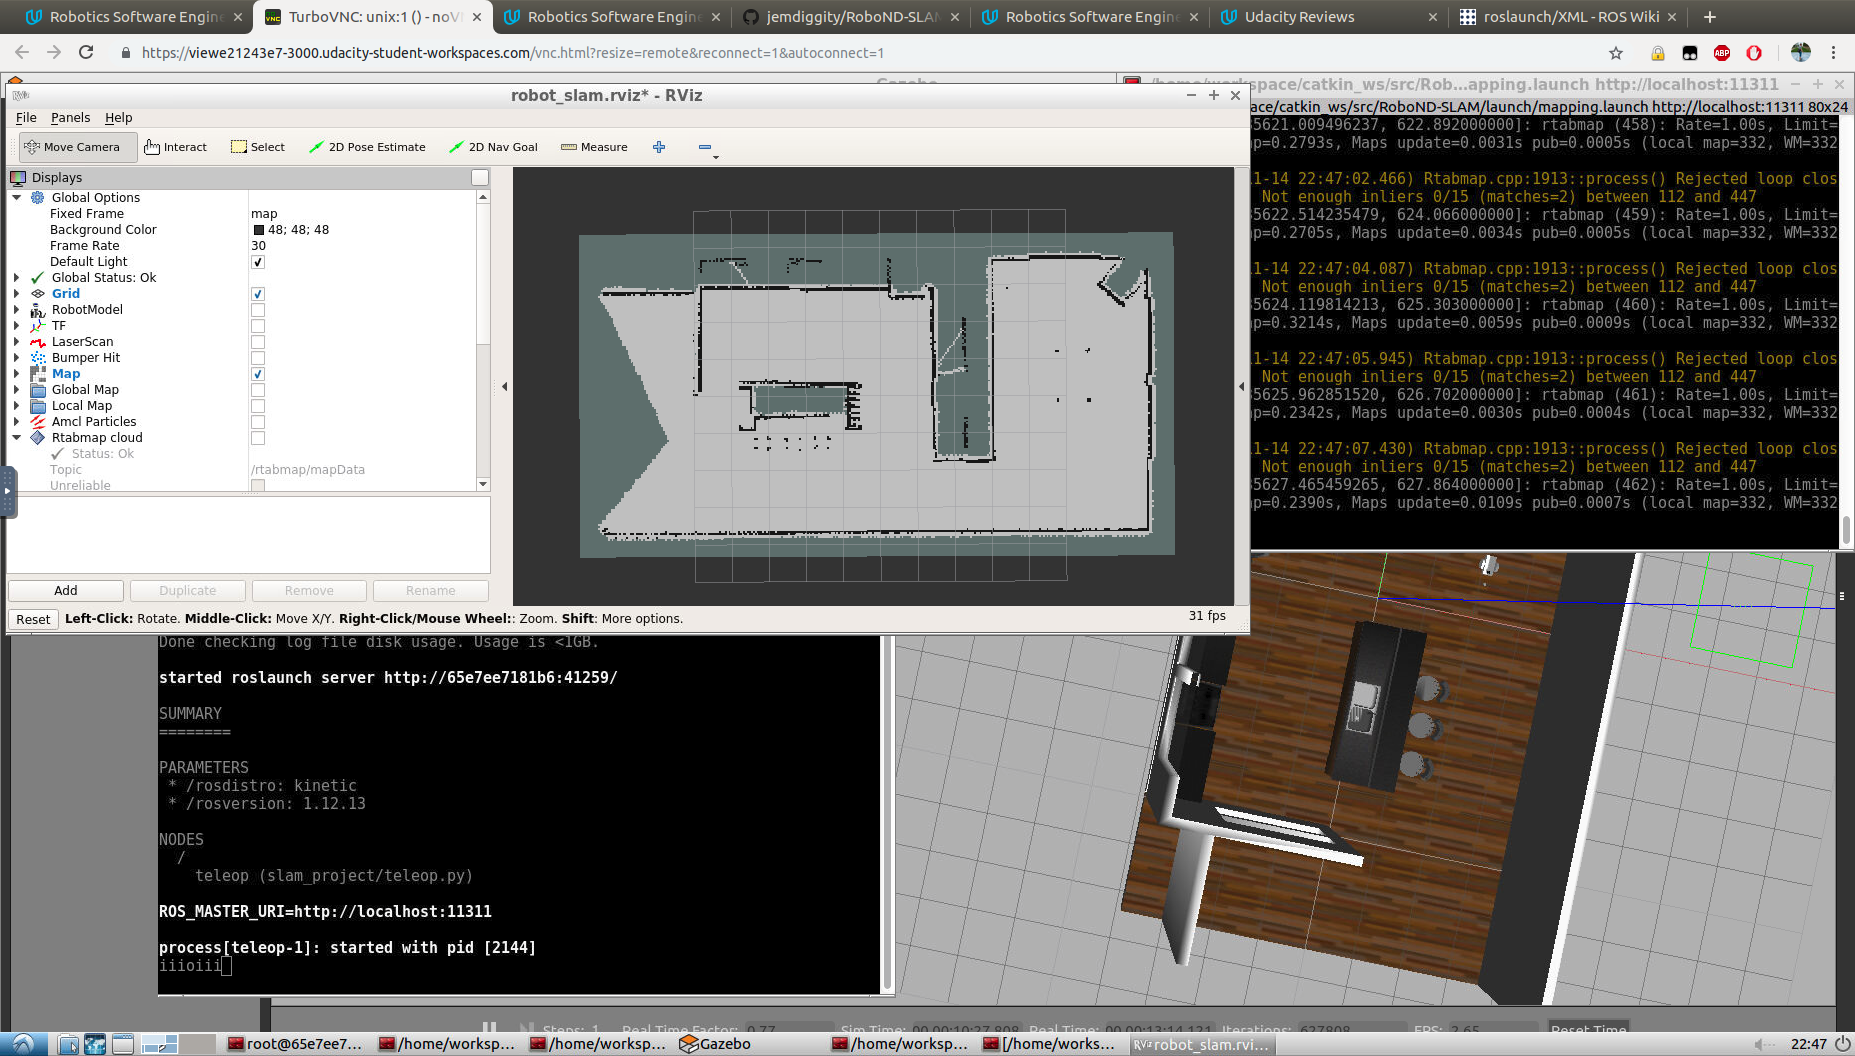
\includegraphics[width=\linewidth]{dining_map}
    \caption{Kitchen \& Dining Occupancy Map}
    \label{fig:dining_2d}
\end{figure}

\begin{figure}
    \centering
    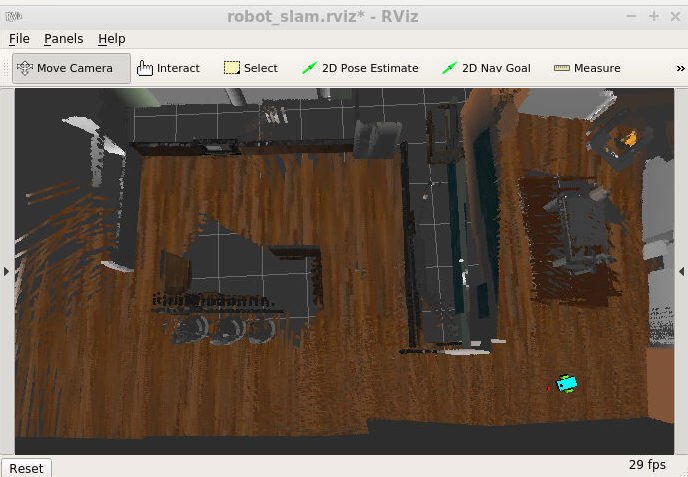
\includegraphics[width=\linewidth]{workspace_benchmark_crop}
    \caption{Kitchen \& Dining 3D Map}
    \label{fig:dining_3d}
\end{figure}

\begin{figure}
    \centering
    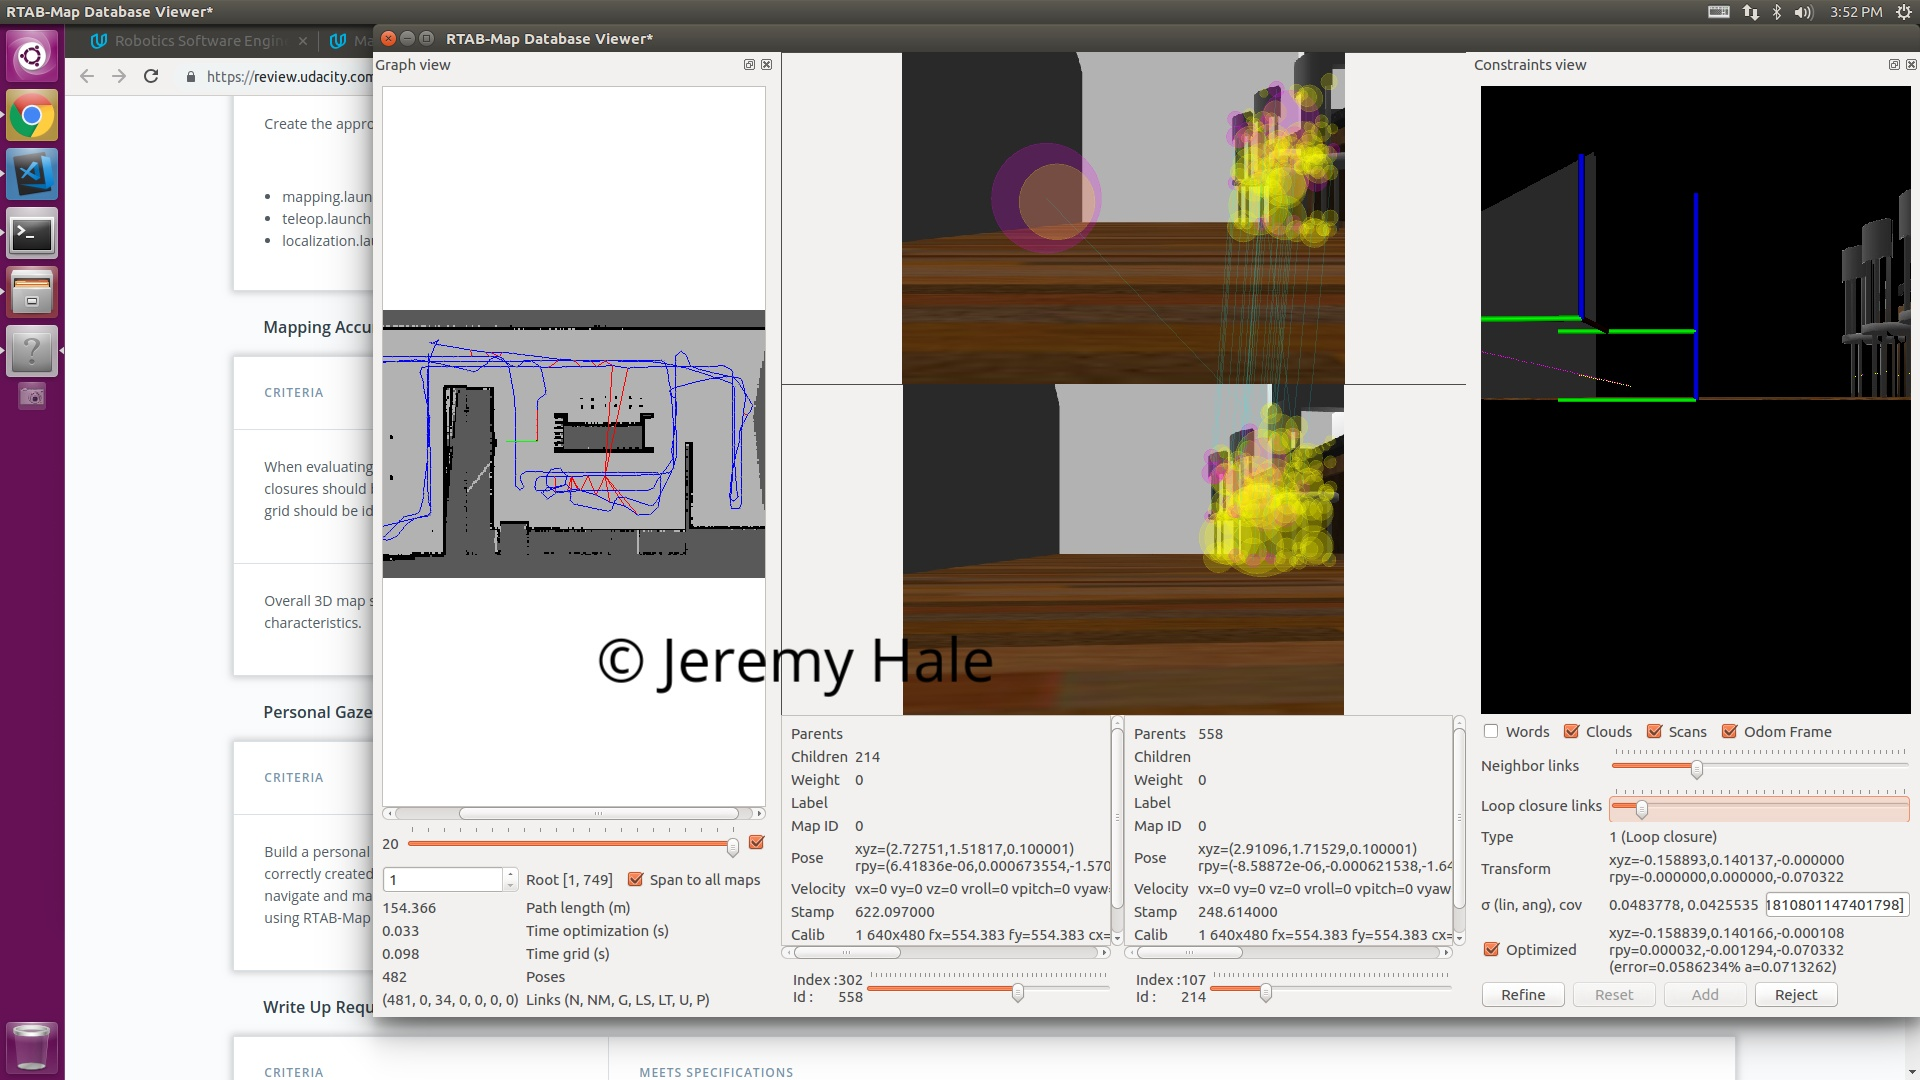
\includegraphics[width=\linewidth]{closure_1}
    \caption{Udacity World Closure}
    \label{fig:closure 1}
\end{figure}

\begin{figure}
    \centering
    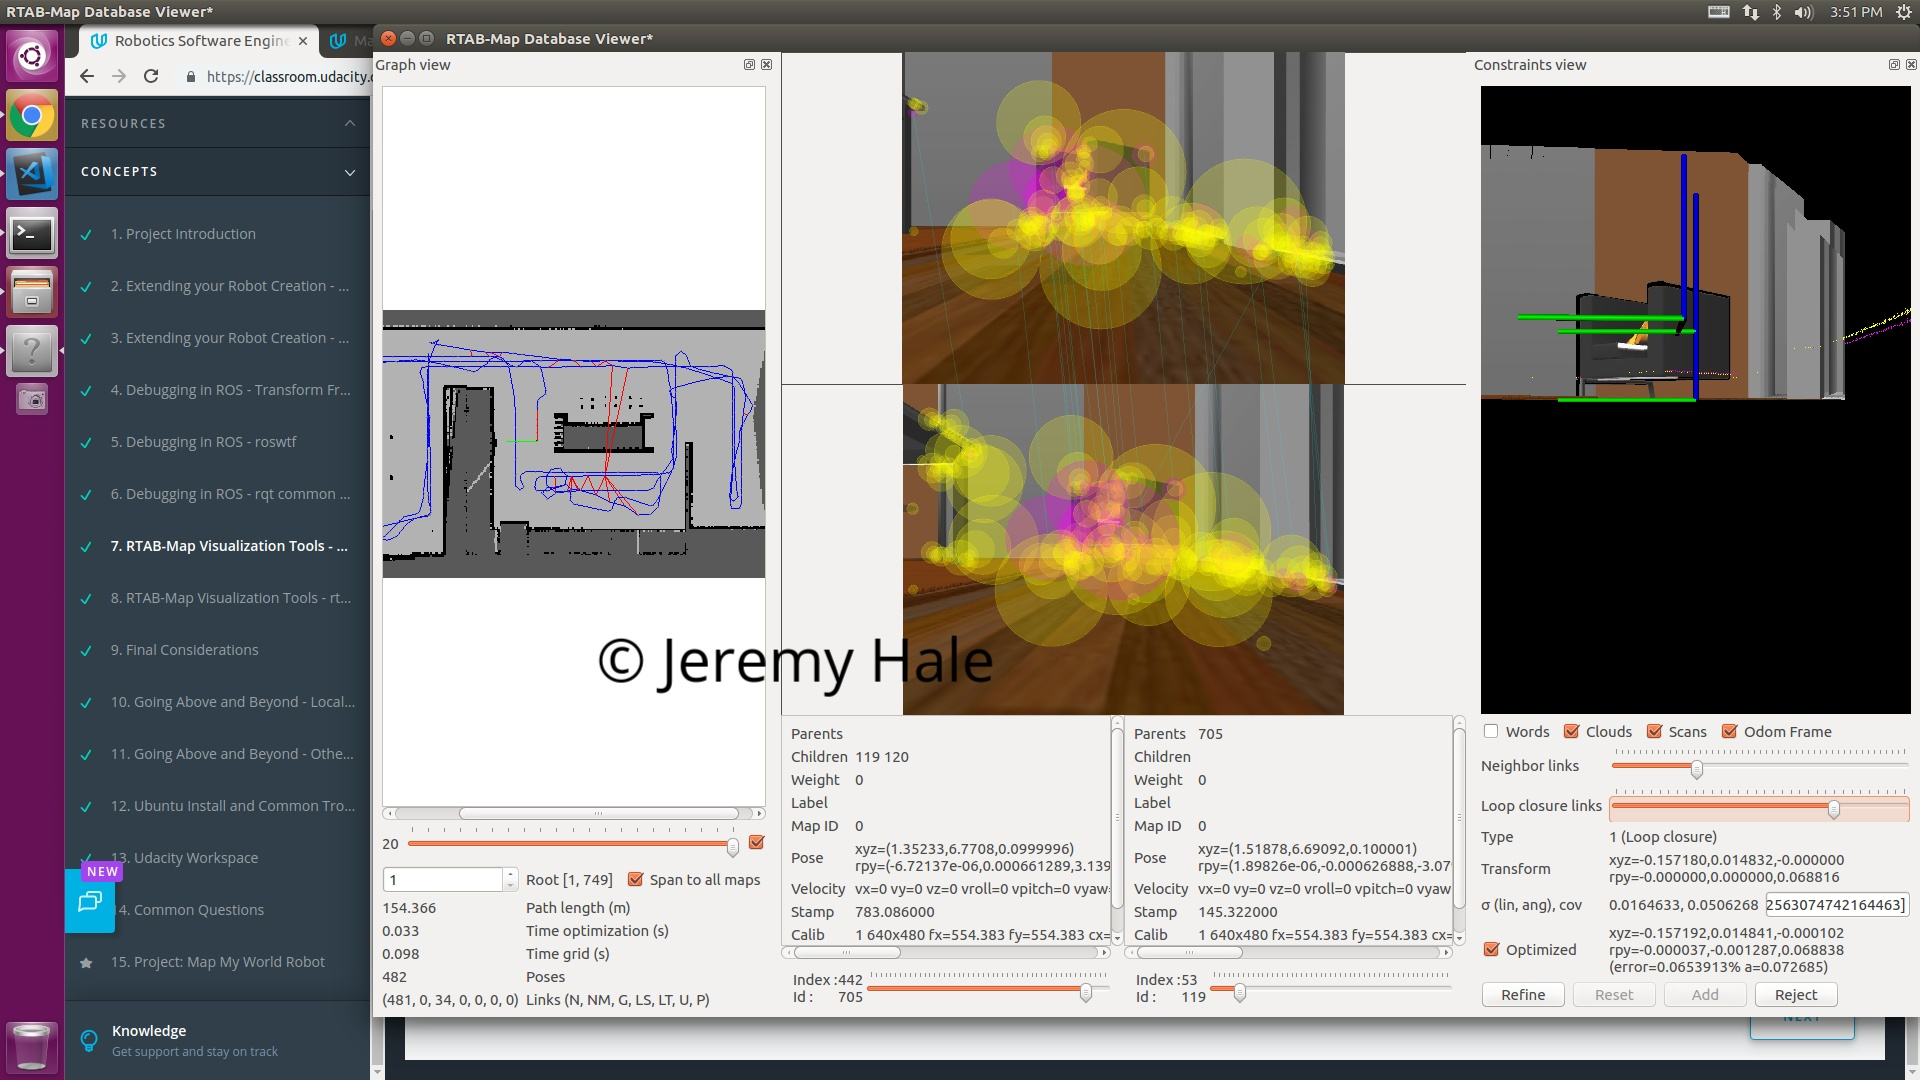
\includegraphics[width=\linewidth]{closure_2}
    \caption{Udacity World Closure}
    \label{fig:closure 2}
\end{figure}

\begin{figure}
    \centering
    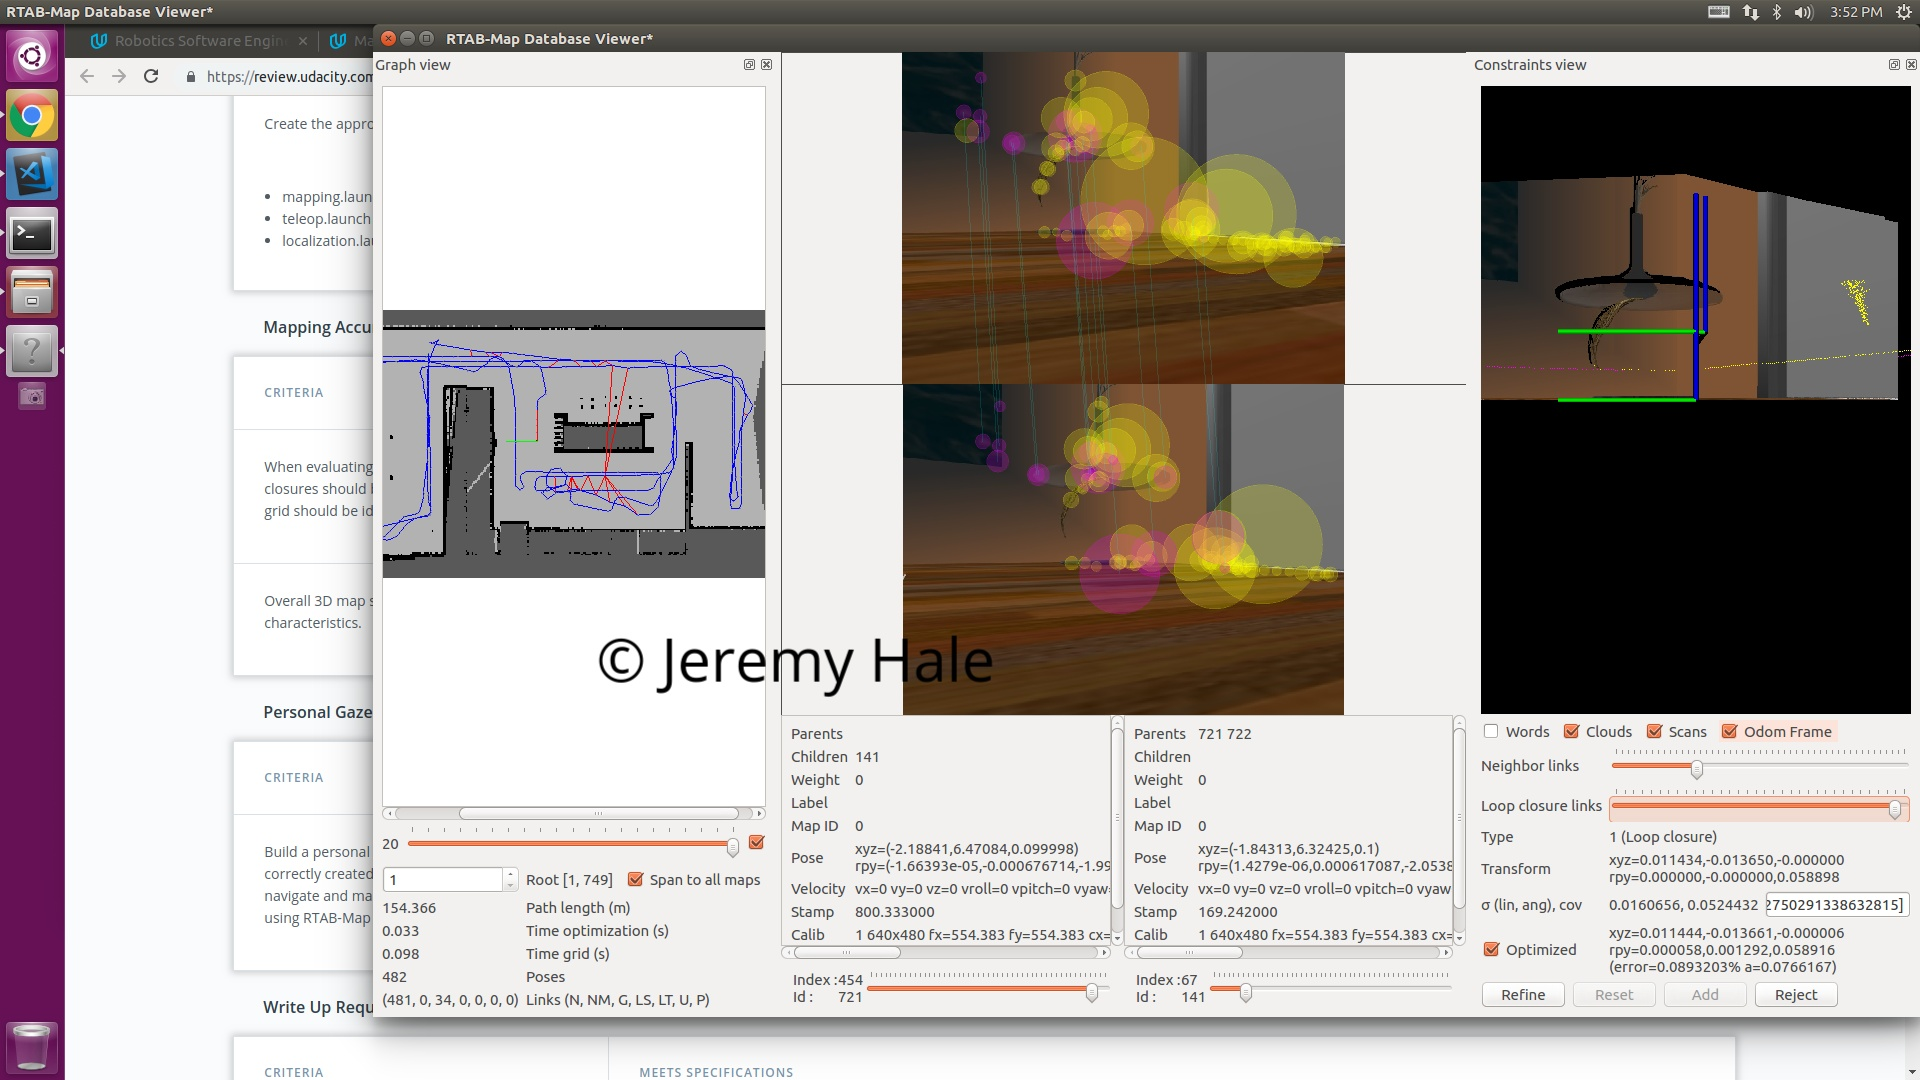
\includegraphics[width=\linewidth]{closure_3}
    \caption{Udacity World Closure}
    \label{fig:closure 3}
\end{figure}

\subsection{Back Alley}

The occupancy and 3D maps for the "Back Alley" world are shown below. There are also images showing the 3 closures.

\begin{figure}
    \centering
    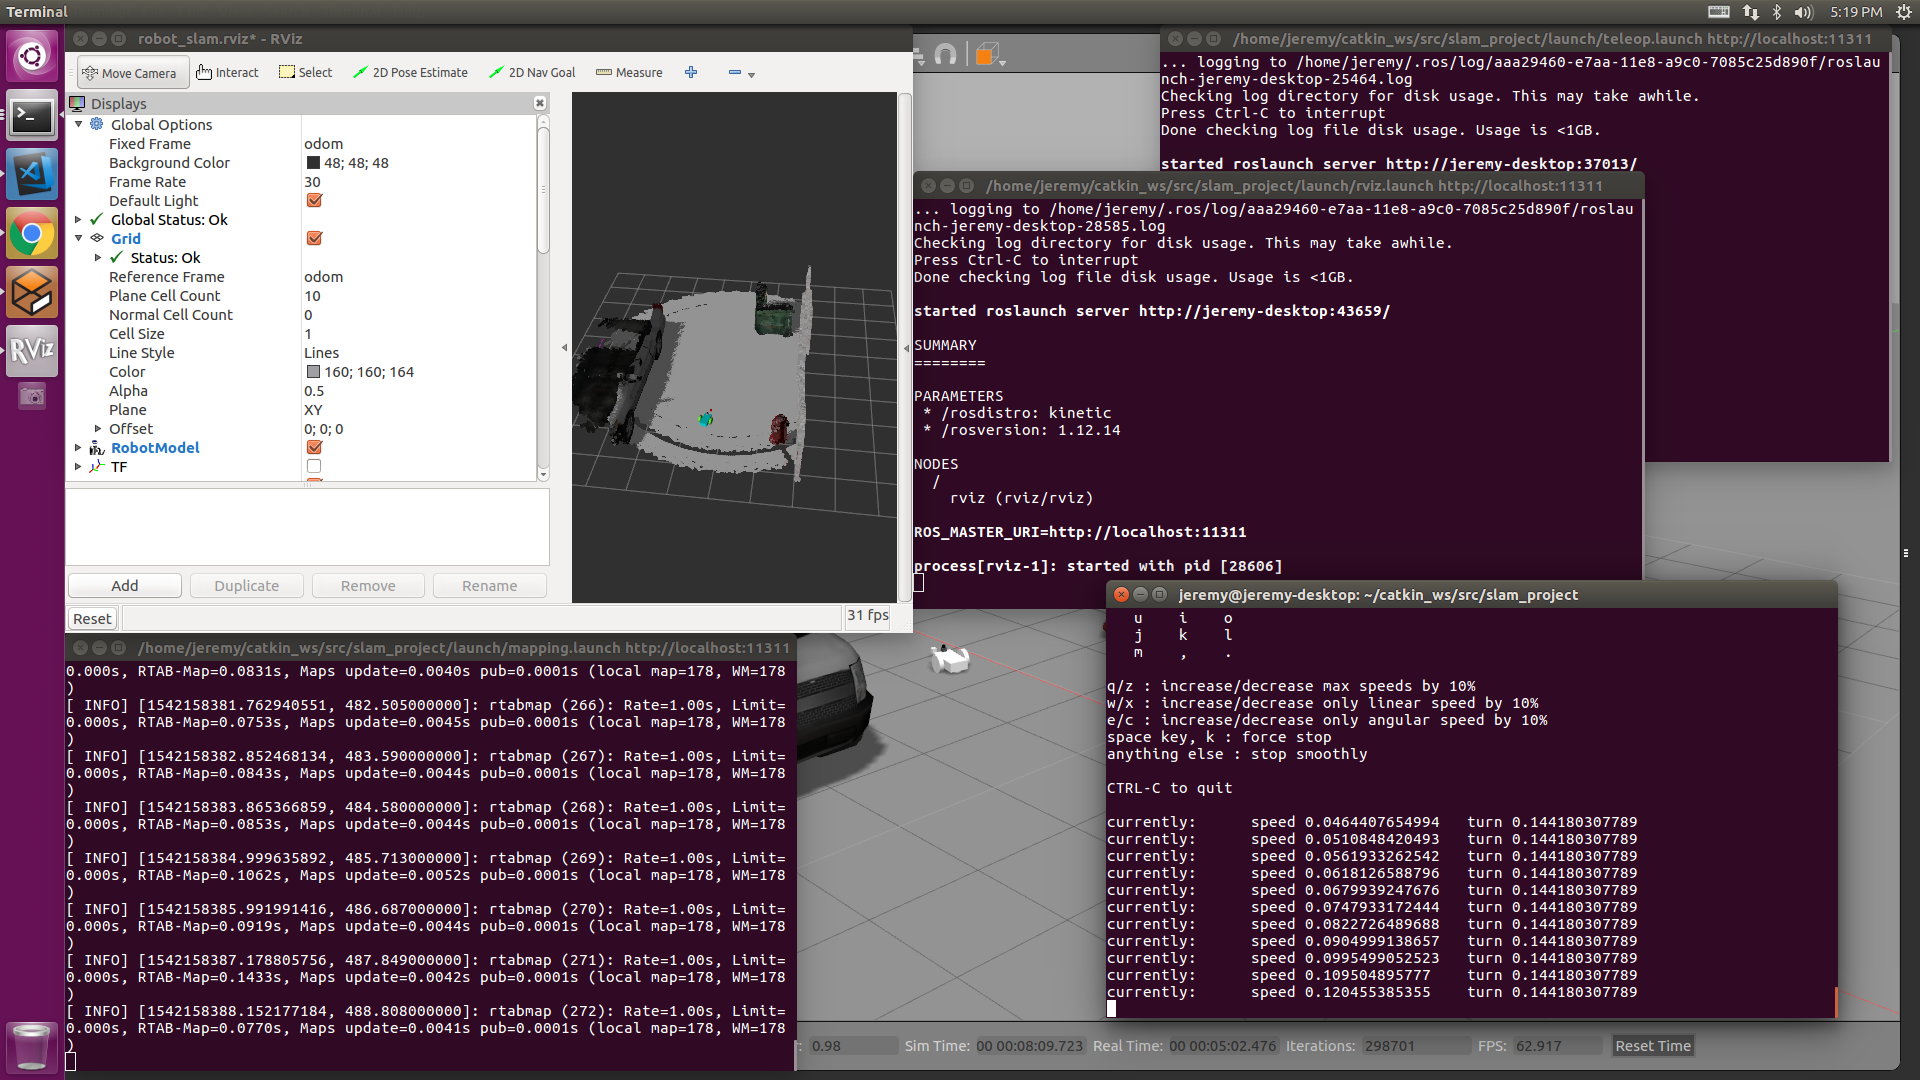
\includegraphics[width=\linewidth]{alley}
    \caption{Back Alley Process}
    \label{fig:alley_process}
\end{figure}

\begin{figure}
    \centering
    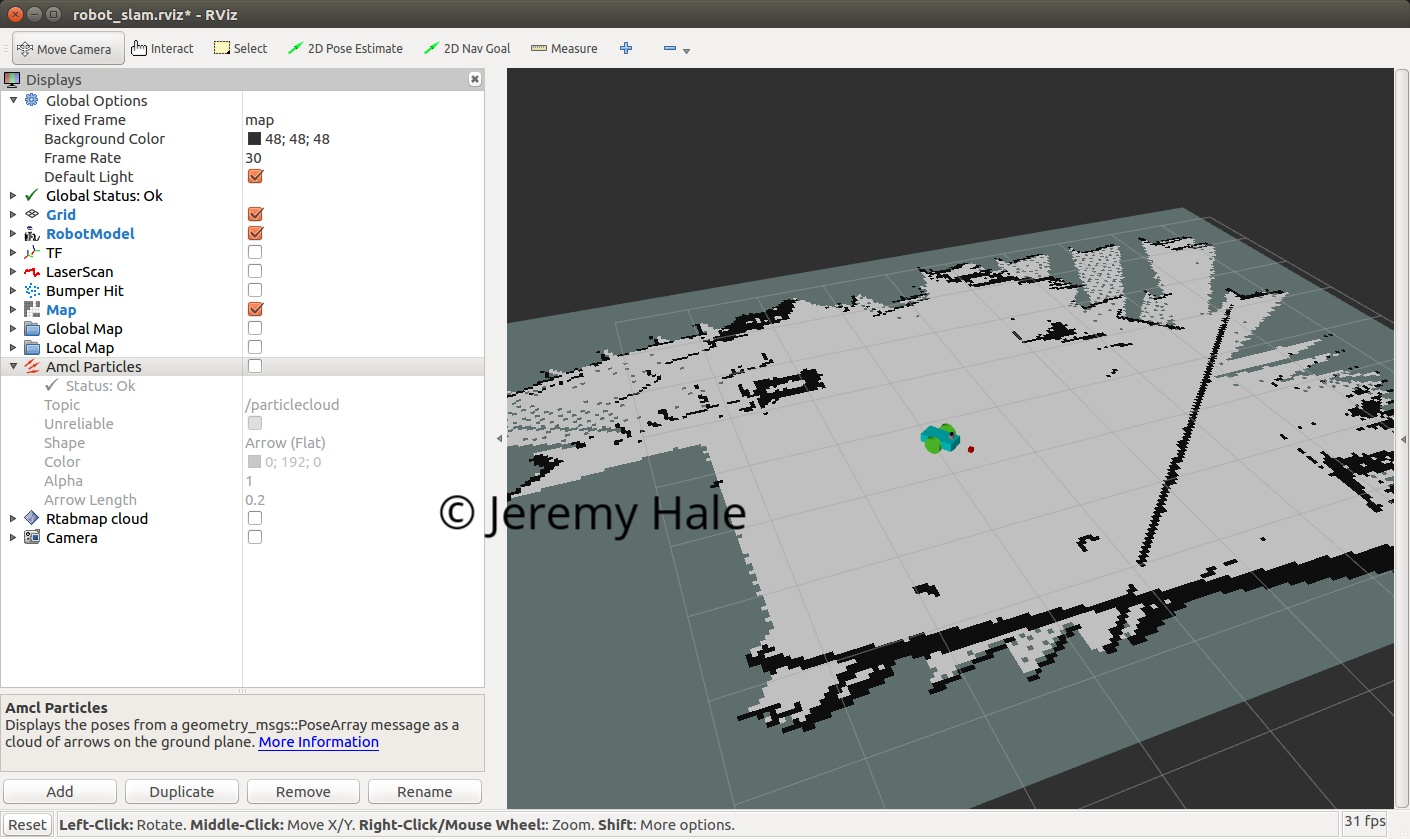
\includegraphics[width=\linewidth]{alley_occupancy}
    \caption{Back Alley Occupancy}
    \label{fig:alley_2d}
\end{figure}

\begin{figure}
    \centering
    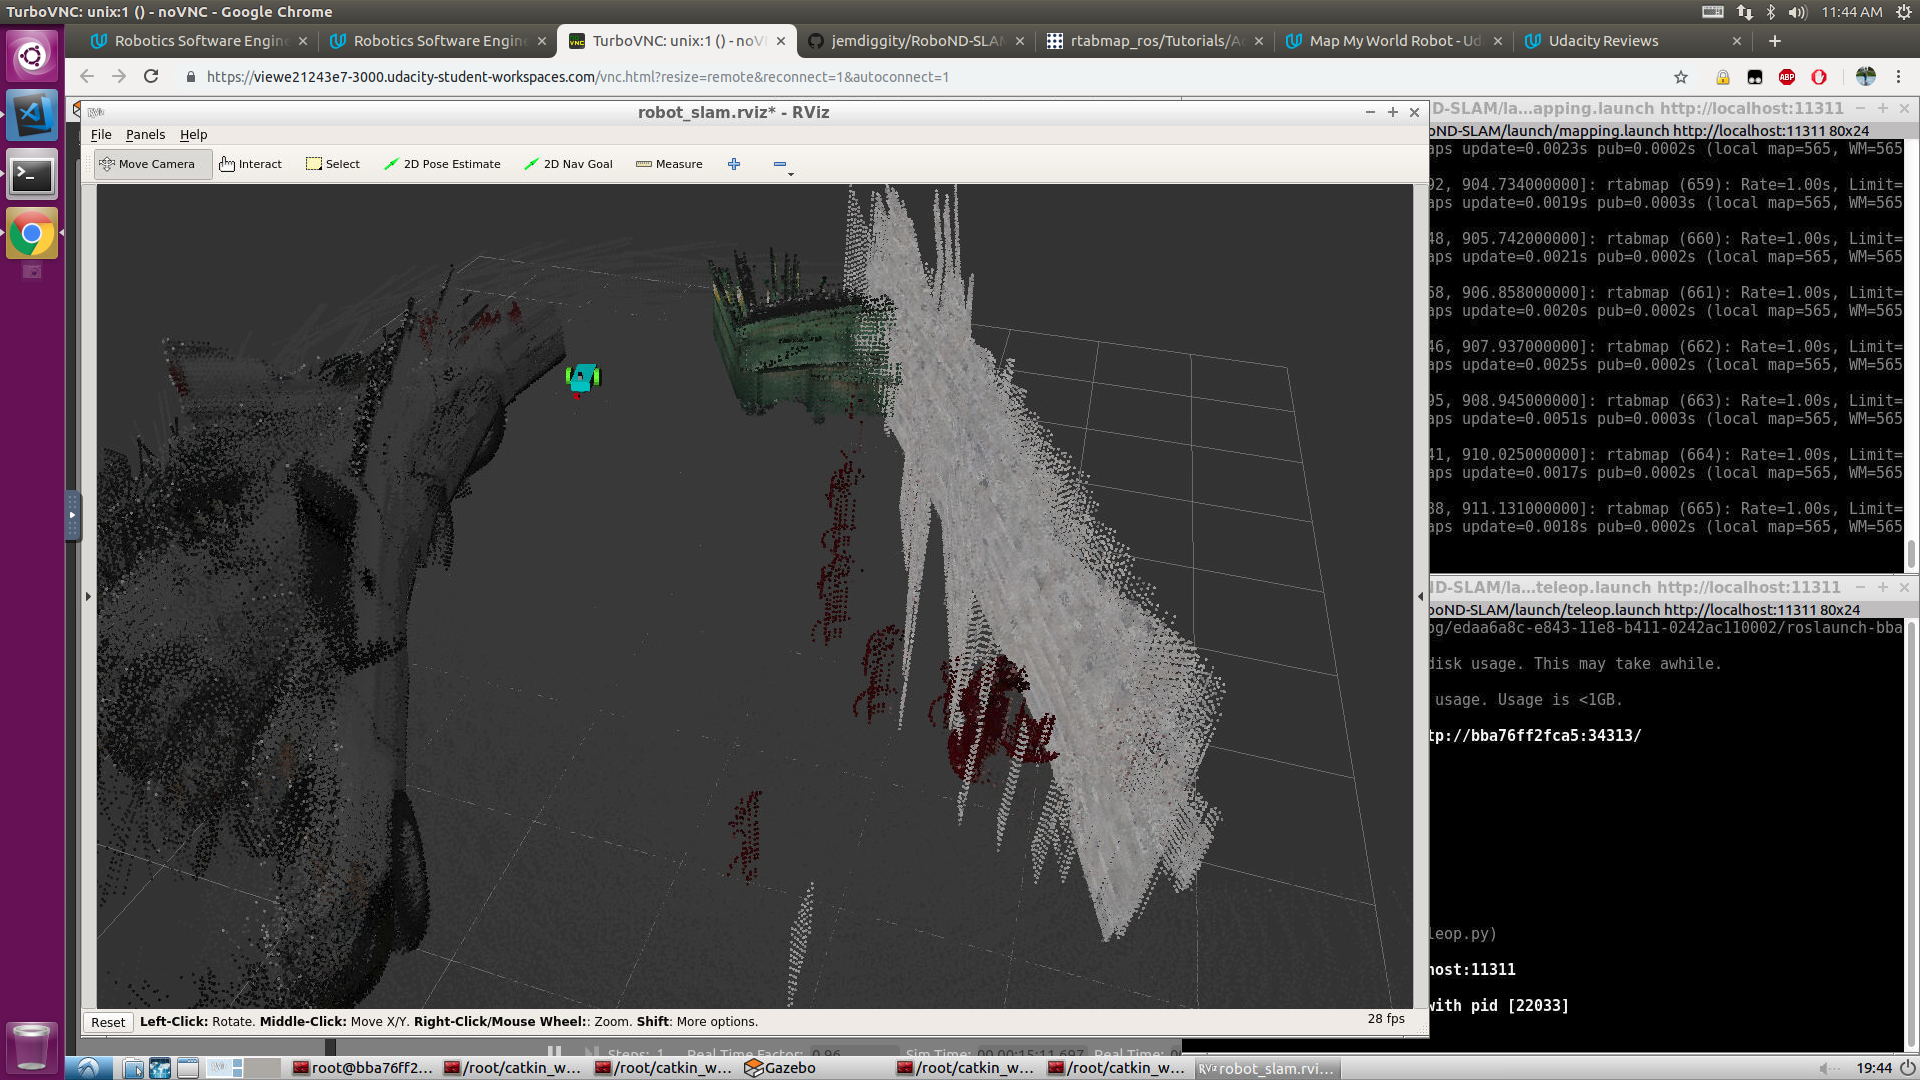
\includegraphics[width=\linewidth]{alley_confused}
    \caption{Back Alley Map}
    \label{fig:alley_3d}
\end{figure}

\begin{figure}
    \centering
    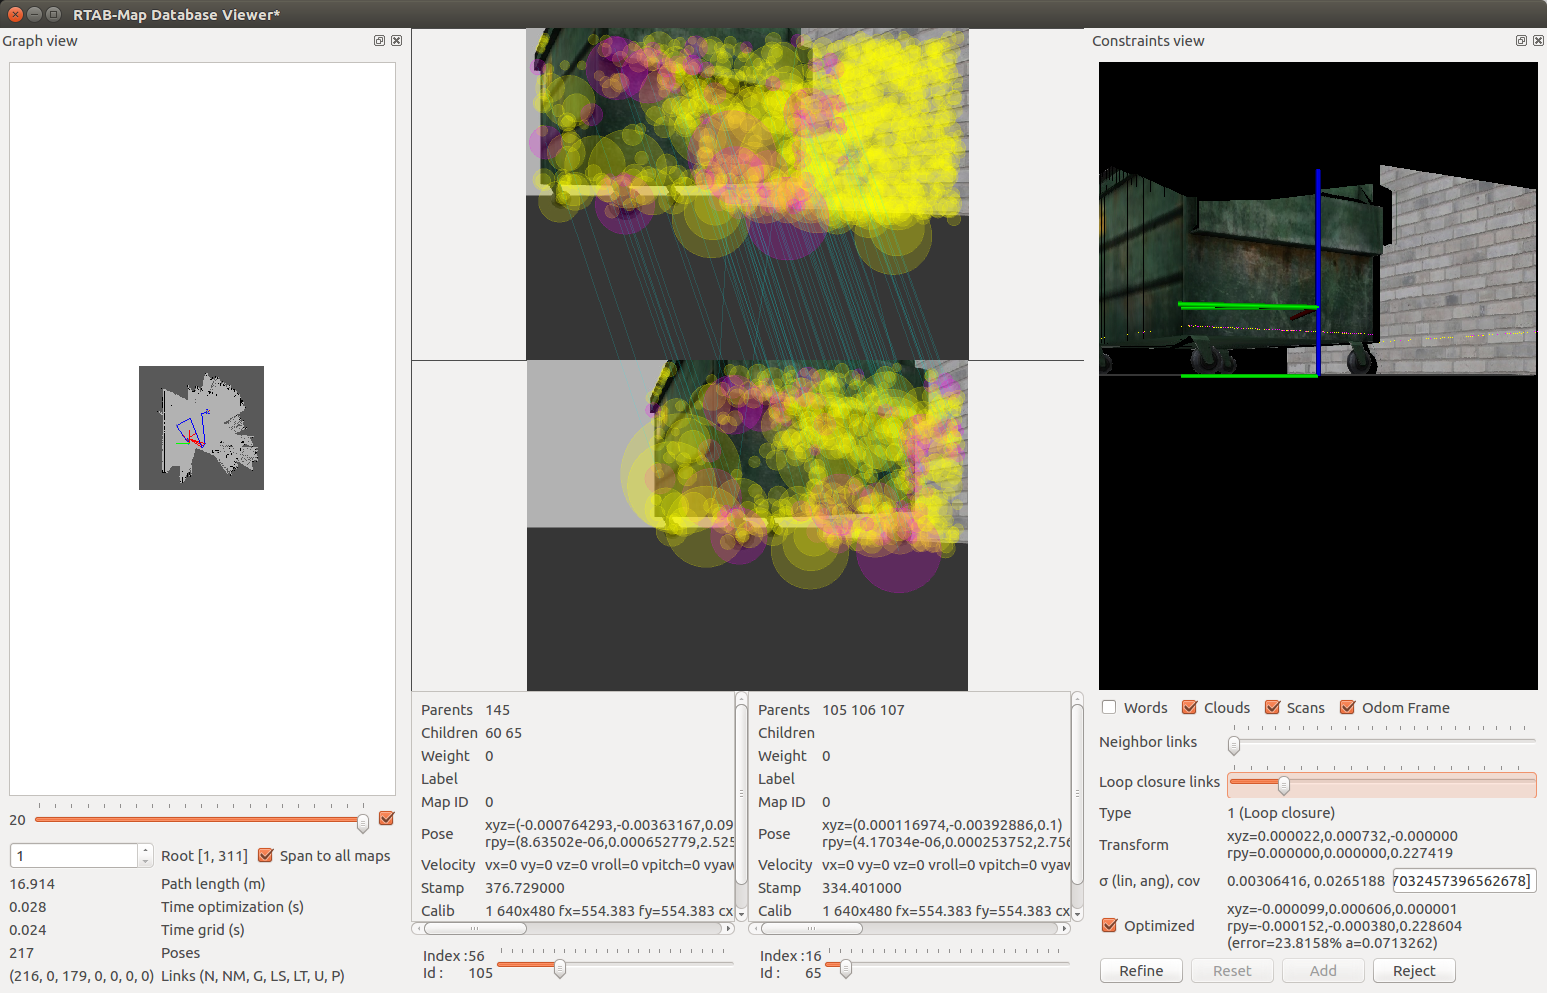
\includegraphics[width=\linewidth]{alley_closure_1}
    \caption{Alley Closure 1}
    \label{fig:alley_closure_1}
\end{figure}

\begin{figure}
    \centering
    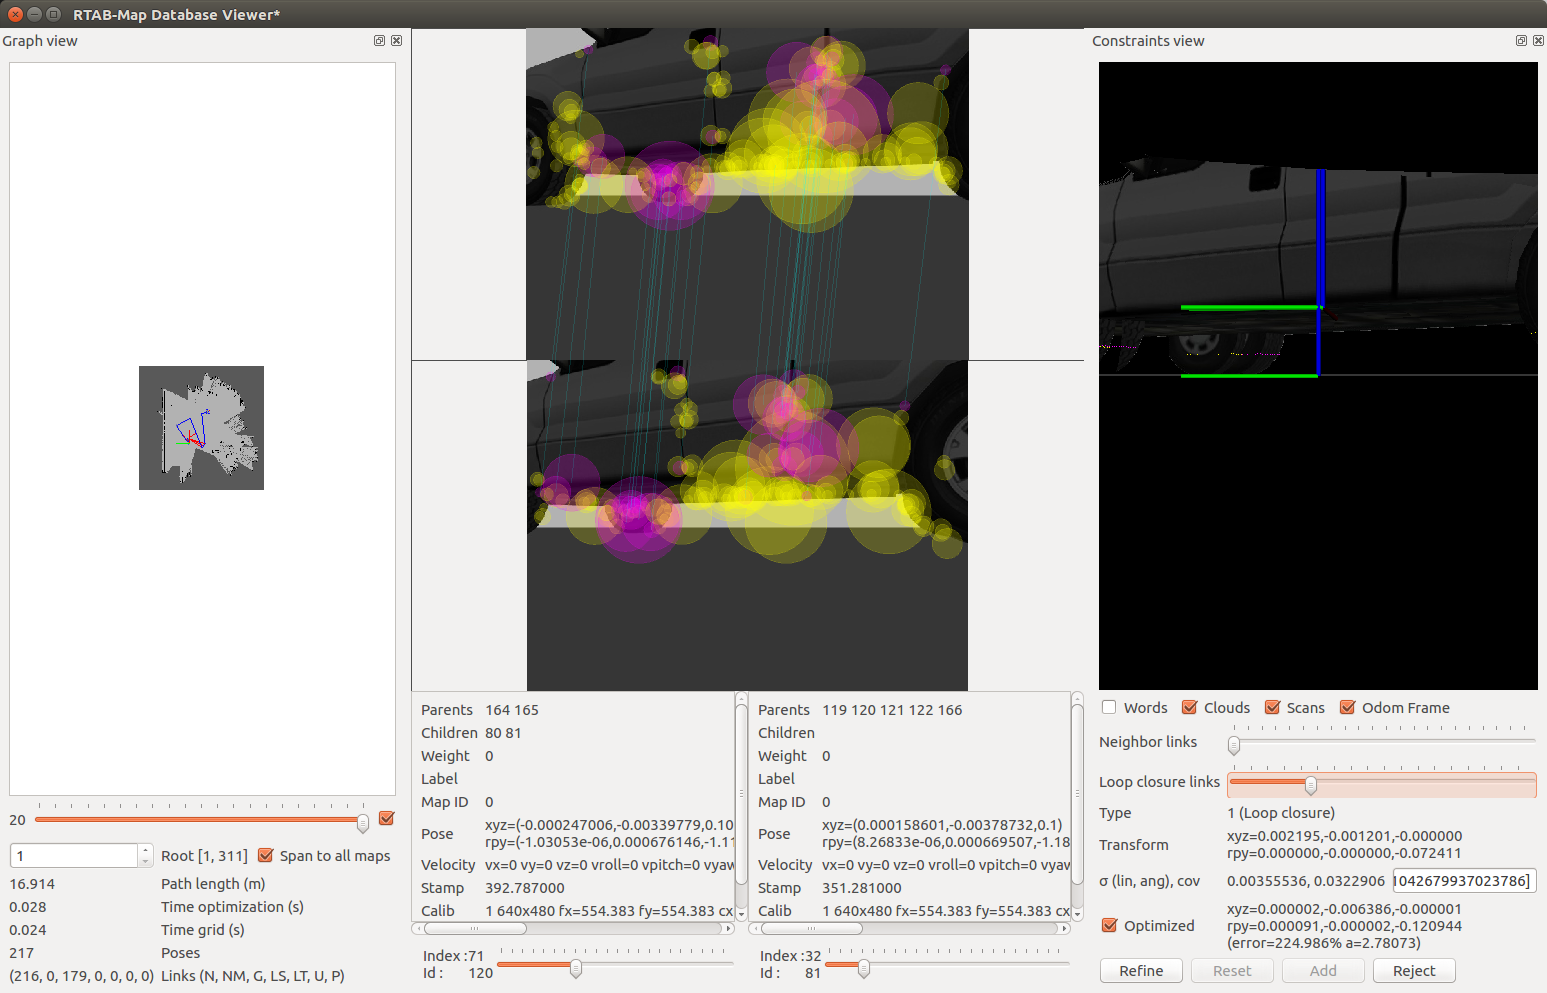
\includegraphics[width=\linewidth]{alley_closure_2}
    \caption{Alley Closure 2}
    \label{fig:alley_closure_2}
\end{figure}

\begin{figure}
    \centering
    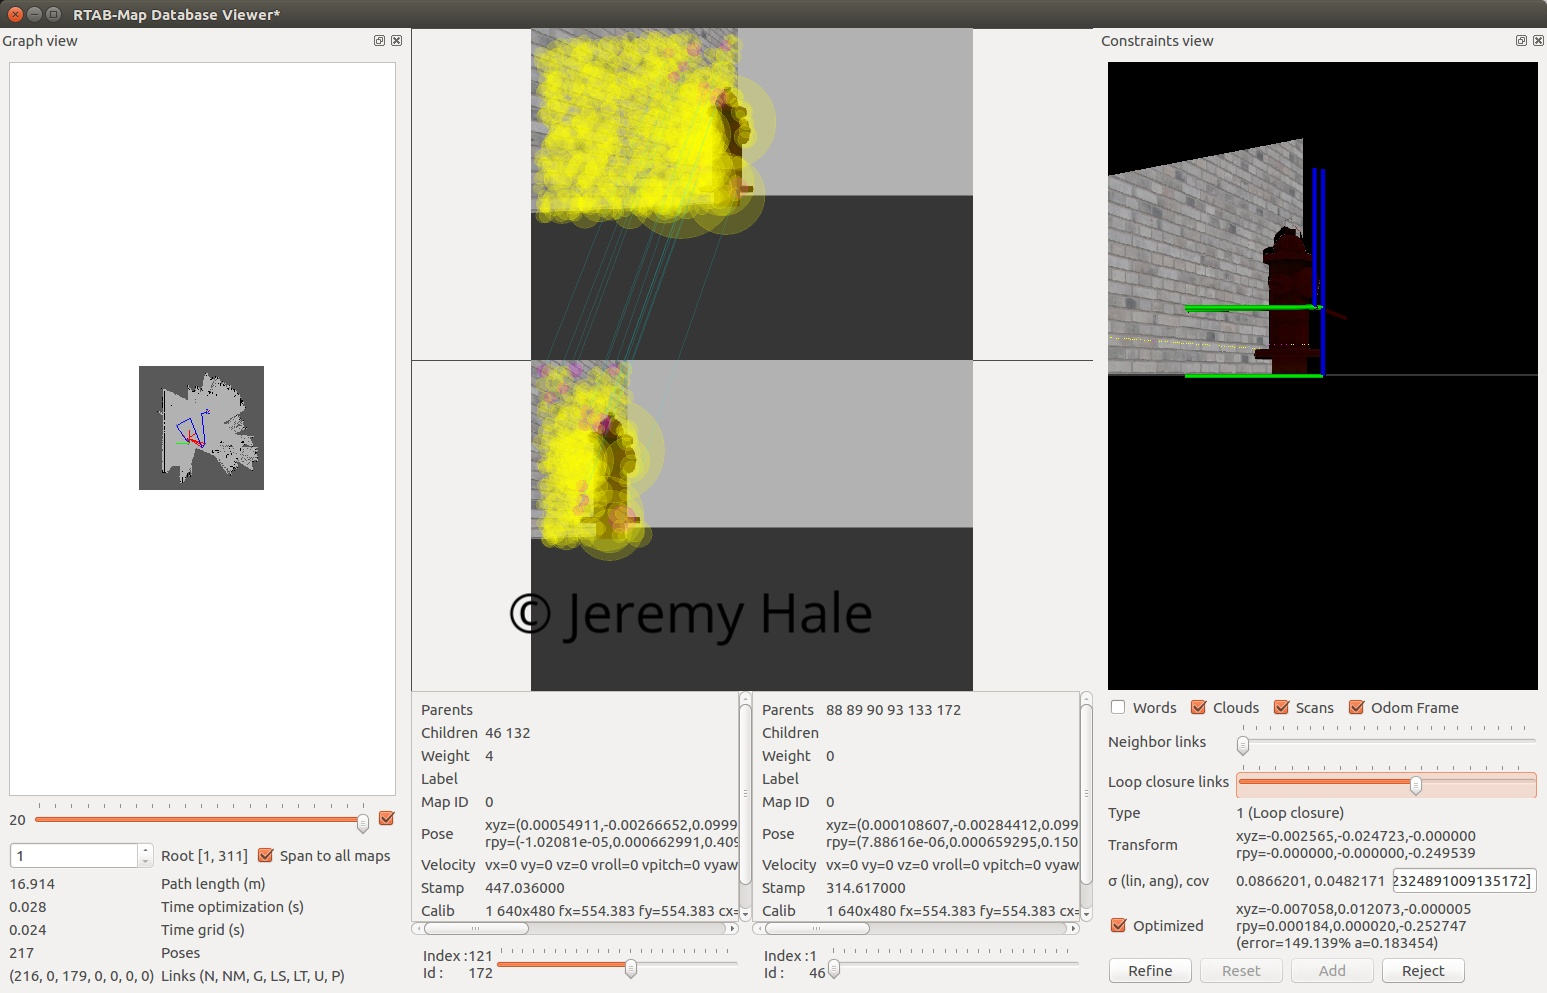
\includegraphics[width=\linewidth]{alley_closure_3}
    \caption{Alley Closure 3}
    \label{fig:alley_closure_3}
\end{figure}

\section{Discussion}
What went well, what went wrong. Reflect upon the results of your robot's performance, and the performance of mapping in both worlds. Justify your answers with facts.

Discussion - The student explains how the procedure went and methodologies to improve it. The student should compare and contrast the performance of RTAB Mapping in different worlds.

\section{Conclusion / Future work}
Student discusses future desires with RTAB-Map. Talk about any robots and environment they applied this too.

"Future Work - The student can discuss how they would like to leverage this tool in robotics. The student identifies other areas where mapping could be done and for what reason. Such as simulated room or physical place.

\bibliography{bib}
\bibliographystyle{ieeetr}

\end{document}